\documentclass[10pt,a4paper]{article}
\usepackage[T1]{fontenc}
\usepackage[utf8]{inputenc}
\usepackage[ngerman]{babel}
\usepackage[a4paper,margin=14mm]{geometry}
\usepackage{lmodern}
\usepackage[table]{xcolor}
\usepackage{tabularx}
\usepackage{amsmath}
\usepackage{microtype}
\usepackage{tikz}
\usepackage{graphicx}
\usetikzlibrary{arrows.meta,calc}
\newif\ifsolution
\solutionfalse
\pagestyle{empty}
\setlength{\parindent}{0pt}
\setlength{\parskip}{0pt}
\renewcommand{\familydefault}{\sfdefault}
\definecolor{Navy}{HTML}{17324D}
\definecolor{Blue}{HTML}{3B6EA5}
\definecolor{Sky}{HTML}{EAF3FA}
\definecolor{Gold}{HTML}{F3B33D}
\definecolor{Ink}{HTML}{1E2935}
\definecolor{Muted}{HTML}{617080}
\definecolor{Line}{HTML}{D8E1E8}
\color{Ink}
\newcommand{\FZ}{F_{\mathrm Z}}
\newcommand{\FG}{F_{\mathrm G}}
\newcommand{\FS}{F_{\mathrm S}}
\newcommand{\kopf}[1]{%
  \colorbox{Navy}{\parbox{\dimexpr\linewidth-2\fboxsep\relax}{%
    \vspace{1.0mm}\color{white}
    \begin{tabularx}{\linewidth}{@{}Xr@{}}
      {\small\bfseries PHYSIK \textperiodcentered{} KLASSE 11} &
      \colorbox{Gold}{\color{Navy}\small\bfseries\strut\ifsolution LÖSUNGEN\else ABFRAGE\fi}
    \end{tabularx}
    \vspace{0.7mm}
    {\fontsize{16}{19}\selectfont\bfseries Aufgabe 6 -- Kräfte beim Kettenkarussell}\par
    \vspace{0.3mm}{\small #1}\vspace{0.8mm}
  }}\par\vspace{0.4mm}}
\newcommand{\frage}[2]{%
  \vspace{0.2mm}{\color{Blue}\bfseries\large #1 \textperiodcentered{} #2}\par
  \vspace{0.1mm}{\color{Blue}\rule{\linewidth}{0.65pt}}\par\vspace{0.5mm}}
\newcommand{\antwortfeld}[2]{%
  \par\vspace{0.4mm}\noindent
  \begin{minipage}[t][\dimexpr9mm*#1\relax][t]{\linewidth}
    \ifsolution
      \vspace*{0.1mm}{\small\color{Blue}#2}
    \else
      \begin{tikzpicture}[x=1mm,y=1mm]
        \foreach \i in {1,...,#1}{\draw[Line,line width=.55pt] (0,{-9*\i}) -- (181.5,{-9*\i});}
        \path[use as bounding box] (0,0) rectangle (181.5,{-9*#1});
      \end{tikzpicture}
    \fi
  \end{minipage}\par}
\newcommand{\fuss}[1]{%
  \vfill{\color{Line}\rule{\linewidth}{0.5pt}}\par\vspace{1mm}
  \begin{tabularx}{\linewidth}{@{}Xr@{}}
    {\small\color{Muted}Klasse 11 \textperiodcentered{} Physik \textperiodcentered{} Kreisbewegungen} &
    {\small\color{Muted}\ifsolution Lösungen\else Abfrage\fi{} \textperiodcentered{} Seite #1 von 2}
  \end{tabularx}}
\newcommand{\vergleichsbilder}{%
\begin{center}\vspace{0.2mm}
\begin{minipage}[c]{0.48\linewidth}\centering
\begin{tikzpicture}[x=1mm,y=1mm,scale=.68,transform shape]
  \path[use as bounding box] (0,-9) rectangle (116,36);
  % Draufsicht: gekrümmte Fahrbahnränder und Pkw von oben.
  \draw[Ink,line width=2.2pt] (2,6) .. controls (36,6) and (42,6) .. (54,15)
    .. controls (66,25) and (82,31) .. (112,31);
  \draw[Ink,line width=2.2pt] (2,0) .. controls (36,0) and (43,0) .. (57,11)
    .. controls (68,20) and (83,25) .. (112,25);
  \draw[Muted,dashed,line width=.6pt] (2,3) .. controls (36,3) and (42.5,3) .. (55.5,13)
    .. controls (67,22.5) and (82.5,28) .. (112,28);
  \node[anchor=west,font=\scriptsize,text=Muted] at (3,33) {Draufsicht};
  \begin{scope}[shift={(54,15)},rotate=38]
    \draw[Ink,fill=Ink,rounded corners=.8pt] (-9,-7.5) rectangle (-5,7.5);
    \draw[Ink,fill=Ink,rounded corners=.8pt] (5,-7.5) rectangle (9,7.5);
    \draw[Navy,fill=Sky,line width=1pt,rounded corners=2pt] (-14,-6) rectangle (14,6);
    \draw[Blue,fill=white,line width=.7pt,rounded corners=1pt] (4,-4.8) rectangle (10,4.8);
    \draw[Blue,fill=white,line width=.7pt,rounded corners=1pt] (-10,-4.8) rectangle (-5,4.8);
    \draw[Muted,line width=.5pt] (-2,-5)--(-2,5);
    \fill[Gold] (12,-4) rectangle (14,4);
  \end{scope}
\end{tikzpicture}
\end{minipage}\hfill
\begin{minipage}[c]{0.48\linewidth}\centering
\begin{tikzpicture}[x=1mm,y=1mm,scale=.68,transform shape]
  \path[use as bounding box] (0,-9) rectangle (116,36);
  \draw[Navy,line width=1.1pt] (52,34)--(52,26);
  \draw[Navy,line width=1.3pt] (30,26)--(52,26);
  \draw[Ink,line width=1.4pt] (30,26)--(68,1);
  % Child: head, torso, arms and legs seated on a small swing seat.
  \fill[Gold] (74,12) circle (4.2);
  \draw[Ink,line width=1.8pt,rounded corners=1pt] (72,8)--(69,2);
  \draw[Ink,line width=1.5pt] (71,6)--(78,3);
  \draw[Ink,line width=1.5pt] (69,2)--(79,1) (69,2)--(66,0);
  \draw[Blue,line width=1.2pt] (64,0)--(82,0);
  \draw[Blue,line width=1pt] (66,0)--(66,-3) (80,0)--(80,-3);
\end{tikzpicture}
\end{minipage}\vspace{0.3mm}\end{center}}
\newcommand{\skizzeparallelogramm}{%
\begin{center}\begin{tikzpicture}[x=.56mm,y=.56mm,>=Latex,font=\small]
  \path[use as bounding box] (0,-5) rectangle (125,63);
  % Rotation axis, boom, chain and seated child.
  \draw[Navy,line width=1.1pt] (20,4)--(20,60);
  \draw[Navy,line width=1.1pt] (13,60)--(27,60);
  \draw[Navy,line width=1.3pt] (20,56)--(61,56);
  \coordinate (H) at (61,56); \coordinate (P) at (85,32);
  \draw[Ink,line width=1.25pt] (H)--(P);
  \draw[Blue,line width=1pt,fill=Sky] (82,29) rectangle (98,23);
  \fill[Gold] (94,35) circle (2.5);
  \draw[Ink,line width=1.2pt] (92,33)--(91,29)--(96,27);
  \draw[Ink,line width=1pt] (91,29)--(86,27) (96,27)--(100,25);
  \draw[Blue] (61,56) ++(0,-8) arc[start angle=-90,end angle=-45,radius=8];
  \node[Blue] at (66,47) {$\alpha$};
  % All three forces share P. The dashed edges close the true force parallelogram.
  \draw[-{Latex[length=2.2mm]},Navy,line width=1.1pt] (P)--(85,8) node[right=1pt] {$\FG$};
  \draw[-{Latex[length=2.2mm]},Blue,line width=1.1pt] (P)--(61,56) node[above left=1pt] {$\FS$};
  \draw[-{Latex[length=2.2mm]},Navy,line width=1.2pt] (P)--(61,32) node[midway,below=1pt] {$\FZ$};
  \draw[Muted,densely dashed,line width=.8pt] (61,56)--(61,32) (85,8)--(61,32);
\end{tikzpicture}\end{center}}
\begin{document}
\kopf{Winkelgeschwindigkeit bestimmen \textperiodcentered{} Kräfte vergleichen}
\frage{1}{Winkelgeschwindigkeit bestimmen}
Auf einen Karussellsitz mit Kind ($m = 65\,\mathrm{kg}$) wirkt bei einem Bahnradius von $r = 4{,}5\,\mathrm{m}$ eine Zentripetalkraft von $\FZ = 2{,}6\cdot10^2\,\mathrm{N}$. \textbf{Berechne} die Winkelgeschwindigkeit $\omega$.
\antwortfeld{6}{$\FZ=m\cdot\omega^2\cdot r$, also $\omega^2=\dfrac{\FZ}{m\cdot r}$ und $\omega=\sqrt{\dfrac{\FZ}{m\cdot r}}$. Mit der positiven Wurzel: $\omega=\sqrt{\dfrac{2{,}6\cdot10^2\,\mathrm N}{65\,\mathrm{kg}\cdot4{,}5\,\mathrm m}}=0{,}942809\ldots\,\dfrac{1}{\mathrm s}\approx0{,}94\,\dfrac{1}{\mathrm s}$. Zwei gültige Ziffern gemä\ss{} Eingabewerten; erst am Ende runden.}
\frage{2}{Auto und Kettenkarussell vergleichen}
\vergleichsbilder
Ein Auto fährt auf ebener Stra\ss{}e durch eine Kurve; ein Sitz mit Kind kreist an schräg gespannter Kette auf gleichbleibender Höhe. \textbf{Erkläre} für beide Fälle, welche realen Kräfte wirken und wie jeweils die zum Kreismittelpunkt gerichtete Zentripetalkraft entsteht.
\antwortfeld{6}{Beim Auto gleichen sich Gewichtskraft nach unten und Normalkraft nach oben aus. Die seitliche Haftreibung der Stra\ss{}e auf die Reifen zeigt zum Kurvenmittelpunkt und liefert die Zentripetalkraft. Bei Sitz und Kind wirken Gewichtskraft nach unten und Seilkraft entlang der schrägen Kette nach oben und zur Drehachse. Ihre vertikalen Anteile gleichen sich aus; ihre waagerechte Resultierende zeigt zur Achse und ist die Zentripetalkraft. Diese ist in keinem Fall eine zusätzliche reale Kraft.}
\fuss{1}
\newpage
\kopf{Auslenkwinkel deuten \textperiodcentered{} Sicherheitsma\ss{}nahme bewerten}
\frage{3}{Auslenkwinkel am Kettenkarussell}
\skizzeparallelogramm
\begin{center}\vspace{-1mm}$\displaystyle\tan\alpha=\dfrac{\FZ}{\FG}$\vspace{-1mm}\end{center}
\textbf{Begründe}, ob der Auslenkwinkel $\alpha$ zunimmt, wenn die Winkelgeschwindigkeit $\omega$ zunimmt.
\antwortfeld{5}{Bei grö\ss{}erer Winkelgeschwindigkeit wird eine grö\ss{}ere Zentripetalkraft benötigt: $\FZ=m\cdot\omega^2\cdot r$; die Gewichtskraft $\FG=m\cdot g$ bleibt gleich. Damit wächst $\dfrac{\FZ}{\FG}=\tan\alpha$, also wird $\alpha$ grö\ss{}er. Der Sitz schwenkt zugleich weiter nach au\ss{}en, wodurch auch sein Bahnradius $r$ zunimmt; dieser ist nicht konstant und verstärkt den Bedarf an Zentripetalkraft. Die Seilkraft und die Gewichtskraft sind die realen Kräfte; $\FZ$ bezeichnet ihre waagerechte Resultierende.}
\frage{4}{Polsterung beurteilen}
{\small \glqq Aufgrund von Sicherheitsbedenken wurde unter den Sitzen im Kinderkarussell auf der Kerwa eine Polsterung angebracht, falls Kinder aus dem Sitz herausfallen sollten.\grqq\par\vspace{0.5mm}}
\begin{center}\vspace{-1mm}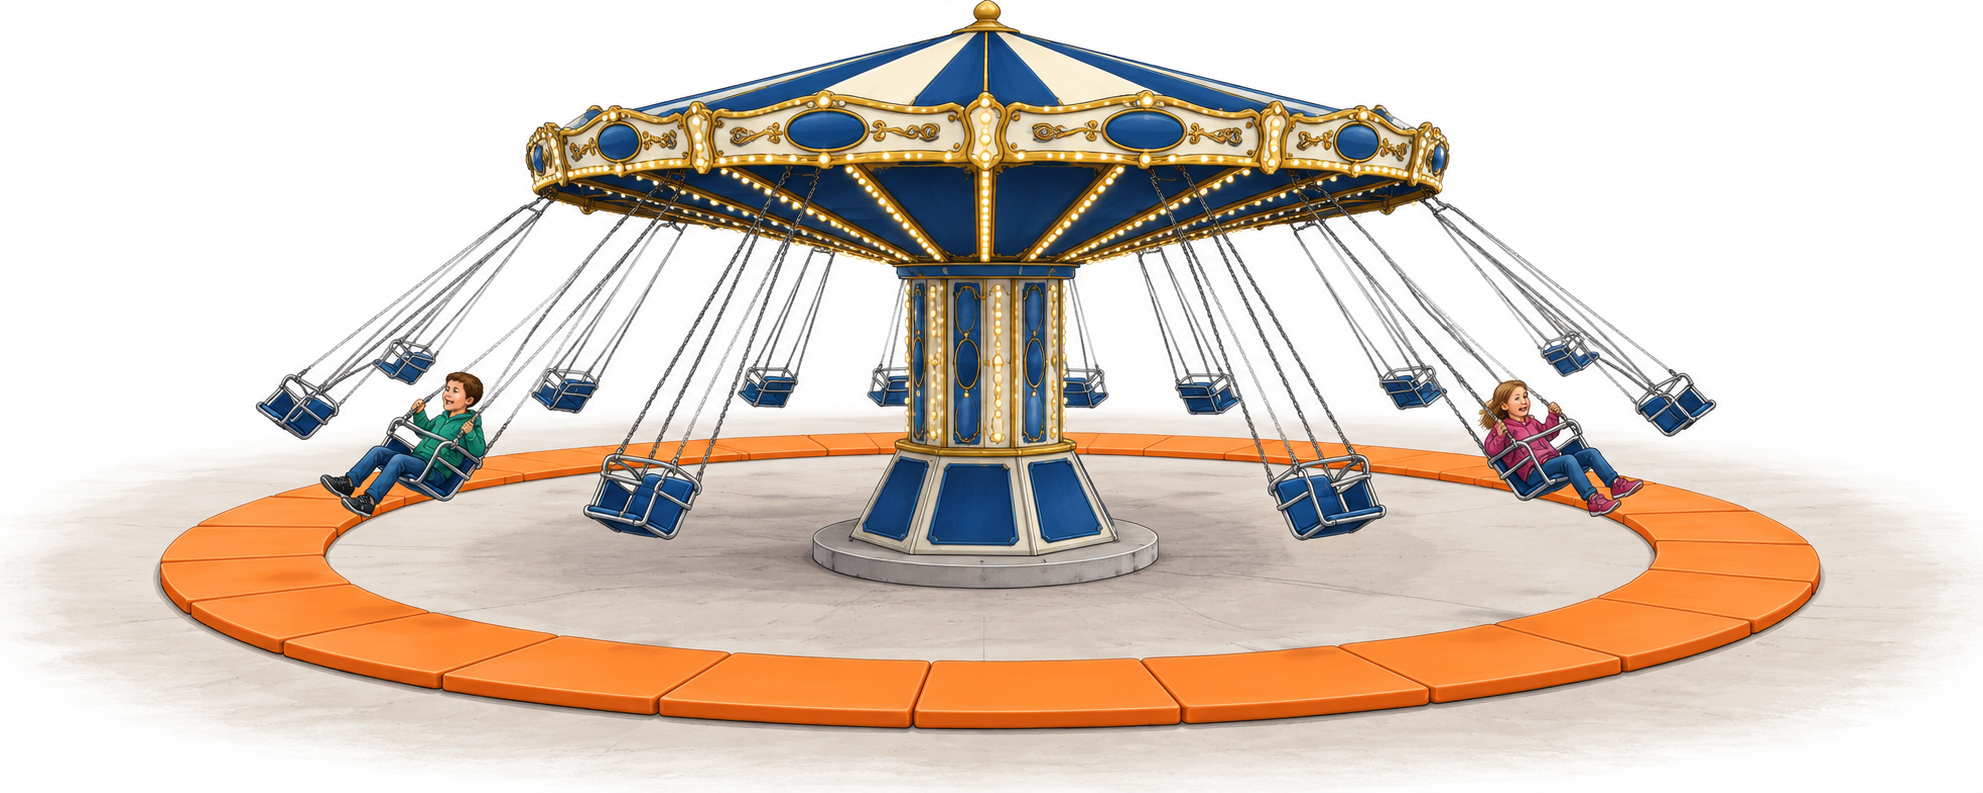
\includegraphics[width=86mm]{../1-Kreisbewegungen/assets/abfrage6-kinderkarussell-polster.png}\vspace{-1mm}\end{center}
\textbf{Bewerte}, ob diese Polsterung einen angemessenen Schutz bietet, falls ein Kind während der Fahrt aus dem Sitz fällt. Begründe dein Urteil mit der Bewegung des Kindes und der Lage der Polster.
\antwortfeld{6}{Die Polsterung kann einen Aufprall abschwächen, wenn ein Kind auf ihr landet. Beim Herausfallen behält es zunächst die tangentiale Geschwindigkeit des Sitzes; zugleich fällt es durch die Schwerkraft nach unten. Es kann deshalb au\ss{}erhalb der begrenzten Polsterfläche aufkommen. Die Polster allein bieten keinen verlässlichen Schutz; sie sind eine ergänzende Ma\ss{}nahme. Eine geeignete Sicherung des Sitzes muss das Herausfallen vorrangig verhindern.}
\fuss{2}
\end{document}
